\label{chap:sprint5}
As in previous sprint chapters, work-flow trough sprint 5 will be described. What makes this sprint different from the others, is that the team had to manage occurred risk on communication module. A good part of this chapter will be devoted to resolution of risk, but it will not lack the rest of the processes such as planning, establishing goals and retrospective.

\section{Sprint planning}

The planning started with customer meeting at Thursday 24th of October 2013. For the customer, the main event and goal of this sprint, is to finalize the prototype and record the demo video. Therefore planning includes tasks as: collecting phones from friends, researching the companies that do mobile development and borrowing the phones from them, renting the room and recording equipment from university. Team agreed to borrow phones from friends, but if that did not work backup plan was to borrow phones from companies.

The recording final demo is planned for Thursday 7th of November, and informing potential phone owners that will be able to share their phones with us is planned at least one week before the event. This way table of potential phones can be created, and risk of not collecting the sufficient number of devices can be reduced and solved. Recording equipment is planned to be rented or reserved at least 3 days before the event.

As far as the implementation is concerned the team focused mainly on device detection part as the customer required to speed up this process. In order to achieve this task the \textit{tree algorithm} for detection was developed (see Section \ref{txt:sprint5_immplementation}). Plan is that the final demo would show an equalizer since the theme for the whole project was a rock concert. Therefore the team also needed to implement a predefined gallery.
In sprint 5 team plan to work further on the report as well to finish sprint 4, start writing sprint 5 and to work further on the evaluation and the conclusion chapters.  

All implementation related stories for sprint 5 are presented in Table \ref{tab:sprint5stories}.
%\caption{User stories selected for Sprint 4.}
  \label{tab:sprint4stories}
 \def\arraystretch{1.25}
 
\begin{longtable}{ccXcc}

\toprule[0.5mm]
\multirow{2}{*}{\textbf{ID}} &
\multirow{2}{*}{\textbf{Ref.}} & \multirow{2}{*}{\textbf{Description}} & \multicolumn{2}{c}{\textbf{Hours}} \\
 					& & & \textbf{Est.} & \textbf{Sp.} \\
%\textbf{ID} 	& \textbf{Description} 	& \textbf{Est.} & \textbf{Sp.} \\
\midrule
\textbf{I4.1} 	& 	& {\bf As a server I need to link the devices' location with their ids.}	 &  52	& \textbf{48} \\

\textbf{I4.2} 	& 	& {\bf As a server I need to identifiy multiple clients from light.}		 &  19	& \textbf{18} \\

\textbf{I4.3} 	& 	& {\bf As a server I need to map all available devices to grid.} 			 & 22 & \textbf{18} \\	

\textbf{I4.4} 	& 	& {\bf As a server I need to play the whole media to the grid.} 			 & 37 & \textbf{34} \\
	
\midrule
		
				&& \textbf{SUM:}		&		130	& \textbf{136}
 \\																			
\bottomrule[0.5mm]
\end{longtable}
 All the documentation related stories for sprint 5 are presented in Table \ref{tab:sprint5Documentationstories}.
%\caption{User stories selected for Sprint 2.}
\def\arraystretch{1.25}
 
\begin{longtable}{ccXcc}
\label{tab:sprint2Documentationstories}\\[-6mm]
\caption{Documentation stories selected for sprint 2}\\[-4mm]
\toprule[0.5mm]
\multirow{2}{*}{\textbf{ID}} &
\multirow{2}{*}{\textbf{Ref.}} & \multirow{2}{*}{\textbf{Description}} & \multicolumn{2}{c}{\textbf{Hours}} \\
 					& & & \textbf{Est.} & \textbf{Sp.} \\
%\textbf{ID} 	& \textbf{Description} 	& \textbf{Est.} & \textbf{Sp.} \\
\midrule


\textbf{D2.1} 	& 
	\refwbs{wbs_documentation}{WBS 8.2}	& {\bf As a student I need to finish the pre-study chapter.} 									& 	12	& \textbf{ 16} \\

\textbf{D2.2} 	& 
	\refwbs{wbs_documentation}{WBS 8.2}	& {\bf As a student I need to finish the planning chapter.} 									& 	10	& \textbf{ 14} \\

\textbf{D2.3} 	&
	\refwbs{wbs_documentation}{WBS 8.2} 	& {\bf As a student I need to finish requirements chapter.} 									& 	30	& \textbf{ 26} \\

\textbf{D2.4} 	& 
	\refwbs{wbs_documentation}{WBS 8.2}  & {\bf As a student I need to finish the architecture chapter.} 								& 	24	& \textbf{ 12} \\

\textbf{D2.5} 	& 
	\refwbs{wbs_documentation}{WBS 8.2}	& {\bf As a student I need to finish sprint 1 chapter.} 										& 	12	& \textbf{ 16} \\

\textbf{D2.6} 	& 
	\refwbs{wbs_documentation}{WBS 8.2}	& {\bf As a student I need to work on the  sprint 2 chapter.} 									& 	16	& \textbf{ 18} \\
%ASK group about this:
%\textbf{360} 	& \refreq{}
%	& {\bf As a student I need to start on the architechture chapter.} 								& 	?	& \textbf{ ?} \\	

								
\hline
				&& \textbf{SUM:}		&		104	& \textbf{102}
 \\																			
\bottomrule[0.5mm]
\end{longtable}
 All the project management related stories for sprint 5 are presented in Table \ref{tab:sprint5storiesProcess}.
%\caption{User stories selected for Sprint 1.}
\label{tab:sprint1storiesProcess}
\def\arraystretch{1.25}
 
\begin{longtable}{ccXcc}

\toprule[0.5mm]
\multirow{2}{*}{\textbf{ID}} &
\multirow{2}{*}{\textbf{Ref.}} & \multirow{2}{*}{\textbf{Description}} & \multicolumn{2}{c}{\textbf{Hours}} \\
 					& & & \textbf{Est.} & \textbf{Sp.} \\
%\textbf{ID} 	& \textbf{Description} 									& \textbf{Est.} & \textbf{Sp.} \\
\midrule

% === Process ==========================
\textbf{326} 	& 
	& {\bf  As a student I have to track effort time} 	& 		16	& \textbf{16} \\
\textbf{345} 	& 
	& {\bf As a student I have attend the weekly meetings with the customer} 	
	& 	22	
	& \textbf{?} \\
		&& Preparation for demonstration	& 2 & ? \\
		&& Demonstration	& 6 & ? \\
		&& Writing minutes 	&  6 & ? \\	
		&& Customer meeting	&  6 & ? \\
		&& Writting minutes	&  2 & ? \\
		
\textbf{327} 	& 
	& {\bf As a student I have to attend the weekly meetings with the supervisor} 	
	& 	12	
	& \textbf{?} \\
		&& Meeting in week I	& 4 & ? \\
		&& Meeting in week II	& 4 & ? \\
		&& Writing minutes from week I 	&  2 & ? \\
		&& Writing minutes from week II	&  2 & ? \\	

\textbf{344} 	&& {\bf As a student I need to attend the team building.} 	& 		7	& \textbf{9} \\
		

\textbf{321} 	&& {\bf As a student I need to participate to lectures about team dynamics. } 	& 		32	& \textbf{25} \\
				&& Course of group dynamics Thu.	&  &  \\
				&& Summary of course and exchange learned.	&  &  \\				
				
\hline
				&& \textbf{SUM:}		&		164	& \textbf{?}
 \\																			
\bottomrule[0.5mm]
\end{longtable}


% hous all in total: Estimated: 235  Spent: 230


\subsection{Duration}
This sprint is 2 weeks long. From 28th of October 2013 to 10th of November 2013. 
Team agreed on the date of presentation and showing the running demo – on Thursday 7th of November 2013.
Estimated velocity is 200 hours since every team member will devote 25 working hours per week.


\section{Sprint goals}

On the end of this sprint team expect to have working, the prove of concept demo. As core modules are finished, team will invest time in tuning existing and implementing some of the supporting functionalities such as: speeding up the detection process  and preparing predefined gallery to be played. Goal for this sprint is also a time sync between server and clients. Reason is bypassing possible network latency, and enabling clients to play the content more precise. 

\section{Architecture}

At first team was thinking about implementing the clock synchronization from scratch. Using one of the popular algorithms as Berkeley algorithm\footnote{\url{http://ieeexplore.ieee.org/stamp/stamp.jsp?tp=\&arnumber=29484}}, and adding additional responsibility to server or client application. 

The Berkeley algorithm requires feedback communication from clients by implementing receiving message system on server. Calculating the time offset on server and adjusting local times on clients. The protocol will have to expended in order to support clock sync communication. Although this approach will work, lot of changes on existing architecture have to be done.

As focus of this project is on proving the concept, and time for big implementation parts or structure changes is not sufficient, team agreed on researching alternative solutions before start implementing. This is also a part of risk management strategy where team have to be careful not to implement things they are not suppose to, according to Table \ref{tab:risks}. Further research has brought the team to Network Time Protocol (NTP)\footnote{\url{https://tools.ietf.org/html/rfc5905\#section-14}}.

Good thing about NTP is that it is used for variable-latency data networks. It was only needed to find application that provide NTP service, and change client code to call this service and determine what is a local time offset before connecting to Digital Lighter server application. In that case, change of existing architecture will be minimal, and it will play only on client application. No server, or protocol will have to be changed.

As solution Time Server\footnote{\url{https://play.google.com/store/apps/details?id=com.icecoldapps.timeserver}} application have been chosen. It will work on same device as Digital Lighter server application, and it will provide same time as Digital Lighter application would.

\subsection{Logical view}
Logical view of added module is shown in Figure \ref{fig:Time_Sync_class }. Class \texttt{SNTPClient} makes call to time server in separate thread, and in \texttt{doInBackground} method retrieve NtpMessage object in order extract exact time from server. \texttt{NtpMessage} represents a NTP message, as specified in RFC 2030\footnote{\url{http://www.rfc-base.org/txt/rfc-2030.txt}}. The message format is compatible with all versions of NTP and SNTP. This class does not support the optional authentication protocol, and ignores the key ID and message digest fields. For convenience, this class exposes message values as native Java types, not the NTP-specified data formats. For example, timestamps are stored as doubles (as opposed to the NTP unsigned 64-bit fixed point format). However, the constructor NtpMessage(byte[]) and the method toByteArray() allow the import and export of the raw NTP message format.

\begin{figure}[h]
	\centering
		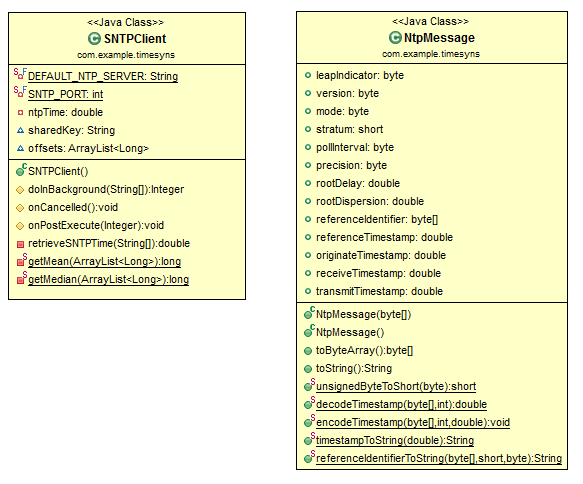
\includegraphics[width=14cm]{sprint5/sprint5_class_diagram.png}
	\caption{Time sync class diagram}
	\label{fig:Time_Sync_class }
\end{figure}

Change have influenced message interchange between server and clients as well. The difference comparing to old sequence diagram is given at Figure \ref{fig:sprint5_sequence_diagram}. New calls are colored red. It is important that time server get started before registering service to the network.

\begin{figure}[h]
	\centering
		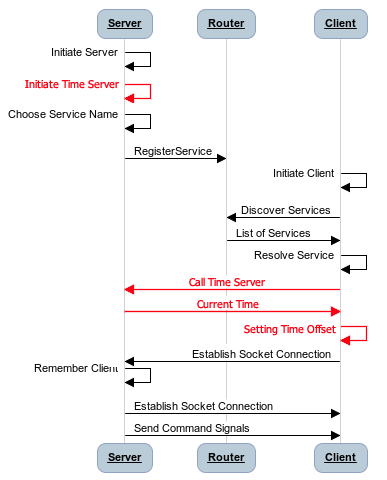
\includegraphics[width=9cm]{sprint5/communication}
	\caption{Sequence diagram}
	\label{fig:sprint5_sequence_diagram}
\end{figure}




\subsection{Physical view}
Deployment digram is also changed, and now includes NTP server as artifact. Additional artifact can be seen on Figure \ref{fig:sprint5_deployment_diagram}

\begin{figure}[H]
	\centering
		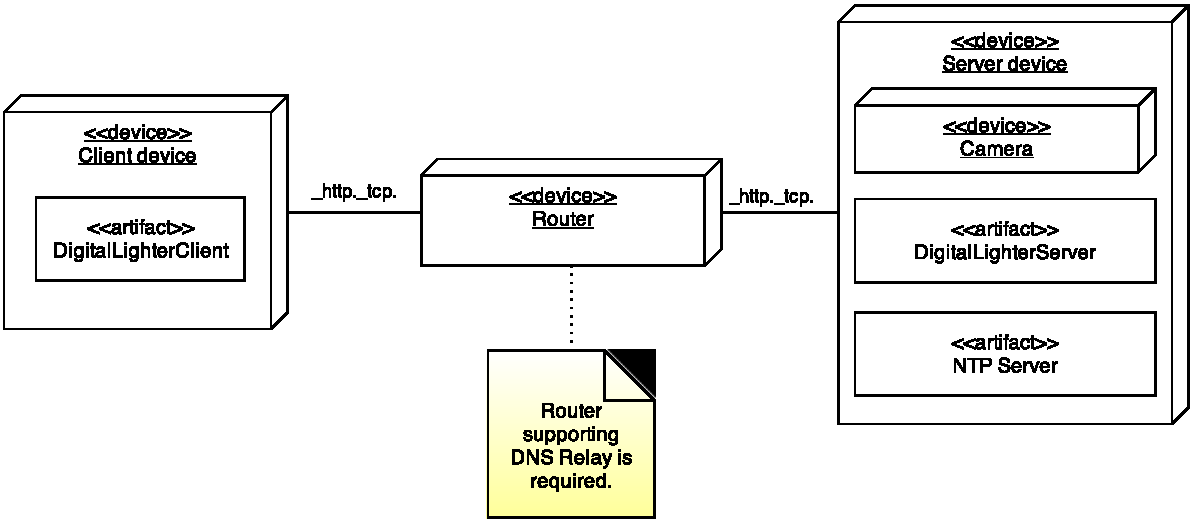
\includegraphics[width=15cm]{images/deployment-diagram-sprint5}
	\caption{Deployment diagram}
	\label{fig:sprint5_deployment_diagram}
\end{figure}



Observing deployment and sequence diagrams, it is easy to see that this solution didn't need existing system to change. But in same time new functionality have been added and big amount of time have been saved.

\section{Implementation} \label{txt:sprint5_immplementation}
This section is devoted to describing the improved algorithm used for faster detection of the devices. So far the simple detection using "one-by-one" approach as explained in Section \ref{txt:sprint4_processview} was used. The drawback of this algorithm is that it performs with time complexity $T(n) = O(n)$ and thus it might get inadmissibly long. Thus more advanced algorithm based on divide and conquer design paradigm was developed. It will be described in greater detail in next sections.

\subsection{Algorithm} \label{subsec:tree_alg}
The algorithm is based on the assumption that the image processing module originally designed and implemented during Sprint 3 (see Section \ref{txt:sprint3_architecture}) is capable of recognizing multiple different colors. Then it possible to recursively divide all the devices into the groups of the same color until there is only one device left in each subgroup. This algorithm is referred to as the \textit{tree algorithm} since the recursive divison gradually creates the tree where each node excluding the leaf nodes has $n$ children where $n = number\_of\_colors\_used\_during\_detection$.

Figure \ref{fig:sprint5_tree_alg} depicts the example of the detection process of the 16 devices while recognizing among 4 different colors: red, green, blue, yellow. In this example the ideal conditions where each device precisely fits into one single matrix tile are set. 

One step of the algorithm can be represented as generating the new level of the tree (STEP 0, STEP 1 and STEP 2 in Figure \ref{fig:sprint5_tree_alg}). Given the specific tree level each node represents the group of devices that are to be lit with the same color. Devices are assigned to the groups randomly and it is required that each group would consist of the the same number of devices if possible (otherwise some groups might differ by 1 device).

Once it was decided which device will be lit by which color the server sends relevant signals to all of the devices and then detects the color blobs in the image. It saves the position of detected colors and proceeds to the next step.

The algorithm ends when there is no more than one device in each color group. Then the saved history of the colors sent to each device can be compared to the actual detected colors and their positions which results in detecting the real position of each device.

\begin{figure}[H]
	\centering
		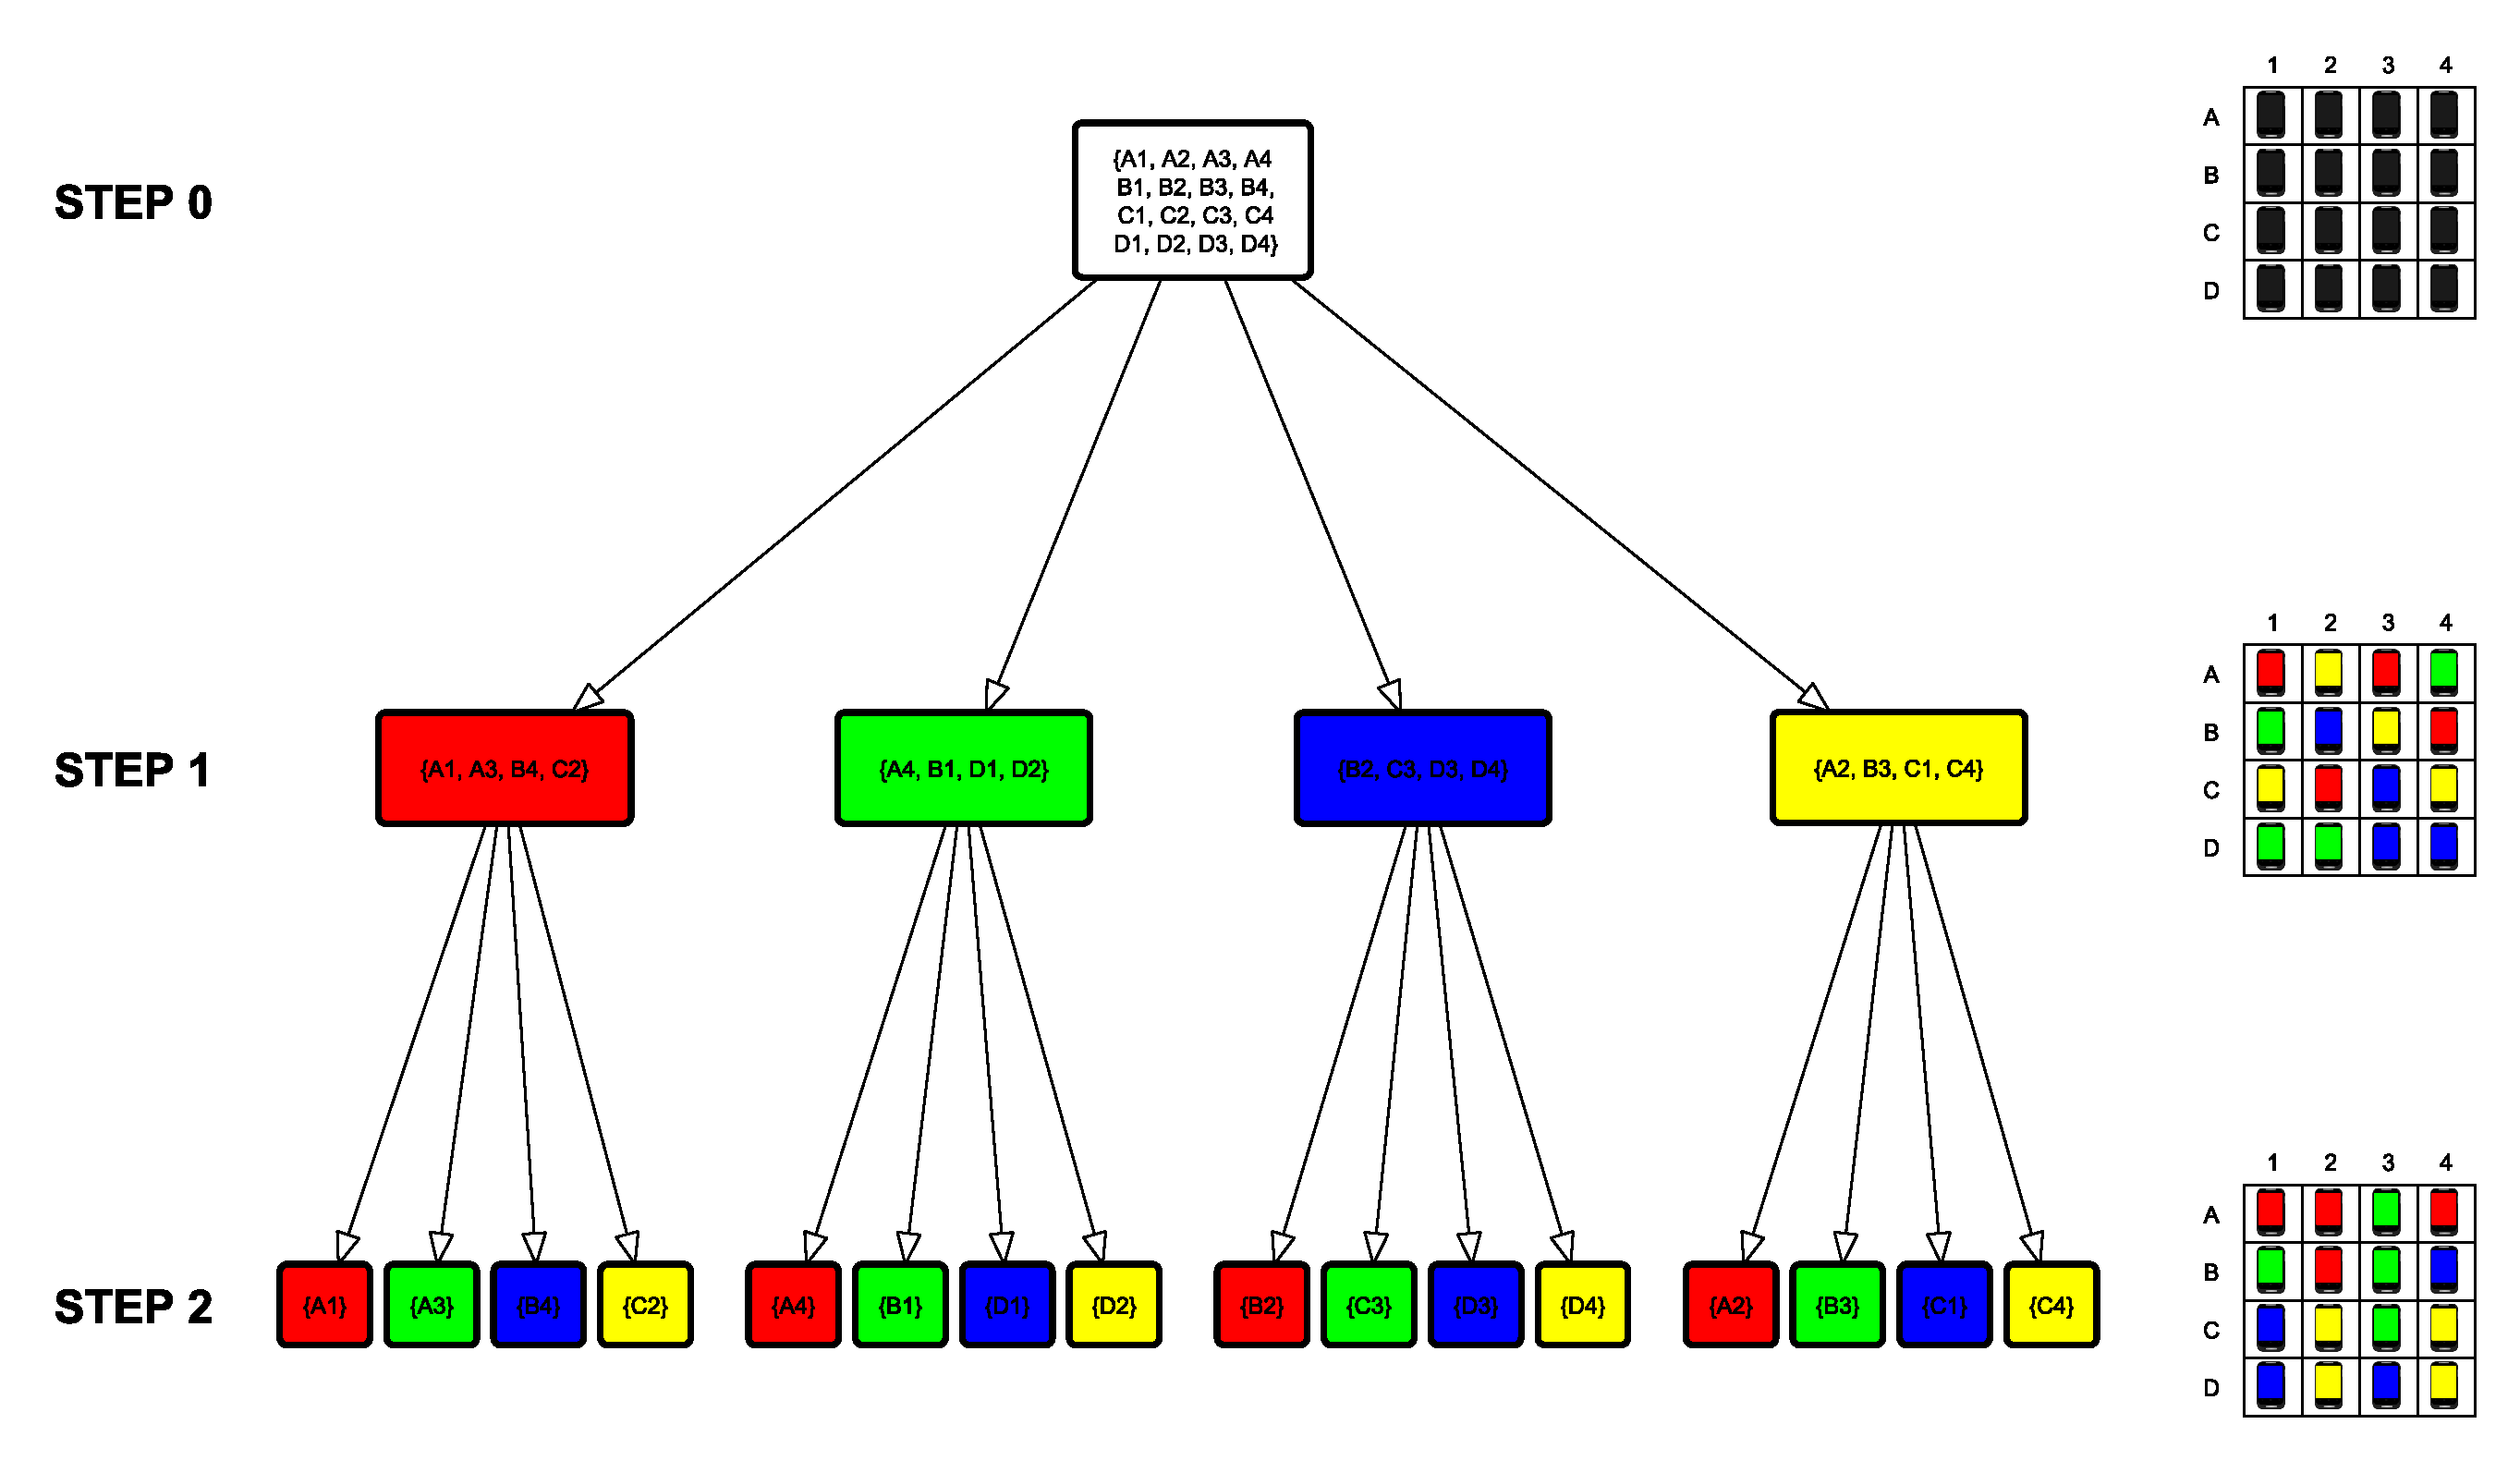
\includegraphics[width=21cm, angle=90]{sprint5/tree_algorithm.eps}
	\caption[Tree algorithm detection example]{Tree algorithm detection example. There are sixteen devices and four detected colors which means it is possible to recognize the position of all devices within two steps.}
	\label{fig:sprint5_tree_alg}
\end{figure}

\subsection{Limitations}
The main drawback of this algorithm is the position resolution. It is only capable of distinguishing between all devices if there are no more than one device in each tile. Otherwise the ambiguities occur and the algorithm finishes in the state where some devices are assigned more then one possible positions.

Nevertheless it has been decided to disregard this issue as this project only serves the purpose of proof of concept and if needed these minor limitations might be improved on performing additional techniques that would solve the problem.

\subsection{Modification}
It might happen that certain devices are not recognized using this algorithm. Therefore this algorithm is accompanied by the former "one-by-one" approach. This fallback option is only invoked if there happen to be devices that failed to being recognized.

\subsection{Performance}
Given the divide and conquer base of this algorithm the time complexity is logarithmic, $T(n) = O(\log n)$, as compared to linear time complexity of the former algorithm. This is though the best-case scenario where all the devices are correctly recognized. In the worst case scenario where no device is recognized during performing tree algorithm the time complexity would be $T(n) = O(\log n + n)$.

\subsection{Communication protocol} \label{sub:comm_protocol_new}
After testing synchronization module it was found that old communication protocol, described in Section \ref{section:impl}, cannot be left unchanged. In order to sync at start or at least during the playing sequence, clients need to receive starting timestamps for every command. This change can be seen on Figure \ref{fig:protocol_5}, with following codding:
\begin{itemize}
\item[] \textcolor{blue!100}{$\bullet$} server time in milliseconds at which client should play specific instruction. Time offset calculated from NTP call is added to this time so all clients can have same value in sum,
\item[] \textcolor{black!100}{$\bullet$} time stamp-color separator,
\item[] \textcolor{red!80}{$\bullet$} color to play(hexadecimal),
\item[] \textcolor{green!100}{$\bullet$} one instruction separator.
\end{itemize}

\begin{figure}[H]
	\centering
		
\includegraphics[width=17cm]{sprint5/protocol_5.png}
	\caption{New command message with multiple instructions.}
	\label{fig:protocol_5}
\end{figure}

\section{Testing}
After adding NTP module some testing considering time synchronization was executed. During this phase there was only 4 devices at team disposal. Details about this devices and their roles can be seen in Table \ref{tab:sp5_test}

\begin{table}[!ht]\centering
\caption{Test devices in sprint 5}
\label{tab:sp5_test}
\def\arraystretch{1.3}
\begin{tabular}{lll}
\toprule[0.5mm]
\textbf{Device} & \textbf{Android os} & \textbf{Role}\\

Samsung Galaxy S2 &  4.1.1 & Router  \\
Samsung Galaxy S3 &  4.1.2 & Server \\
HTC Desire & 2.3 & Client  \\
Samsung Google Nexus S & 4.1.1 & Client \\
\bottomrule[0.5mm]
\end{tabular}
\end{table} 

\paragraph{Test case:}
\begin{enumerate}
\item Start router. Since no real device is available emulate router functionality with one of the phone's tethering option. Name the hot-spot "Sprint5". 
\item Connect server device to the network "Sprint5".
\item Start NTP time server on server device.
\item Start Digital Lighter server application.
\item Name service "testSprint5" and register it to the network.
\item Connect client device to the network "Sprint5"
\item Refresh list of available services on network and select service "testSprint5".
\item Connect to selected service.
\item Repeat steps 6-8 for all client devices.  
\item Choose syncMedia\footnote{syncMedia - media, when played all client devices blink synchronously at given frame rate.} and set frame rate to 2.
\item Detect all present clients and play media.
\item Observe client applications behavior.
\end{enumerate}


\paragraph{Expected server behavior:}
\begin{enumerate}
\item When started, Time Server application, stays as notification icon on notification bar.
\item When service is registered, Toast\footnote{\url{http://developer.android.com/guide/topics/ui/notifiers/toasts.html}} message of confirmation is displayed - "testSprint5 is registered".
\item When clients connect, text label representing number of connected devices will increment.
\item When client device is detected grid square in which device is detected will light up.
\end{enumerate}


\paragraph{Expected client behavior:}
\begin{enumerate}
\item When list of available services is refreshed, all services should be visible in list view.
\item When "testSprint5" service is selected, the Toast message of confirmation is displayed - "testSprint5 service selected".
\item When "Connect" button is pressed, Toast message of confirmation is displayed - "Connected".
\item Few seconds after being connected, Toast message of background synchronization process should be displayed - "Time diff: SOME\_VALUE". Where SOME\_VALUE is client time offset comparing to Time Server.
\item When instructed to play, all clients should blink 2 times per second synchronously. 
\end{enumerate}

\paragraph{Test 1-7 } observed behaviors:
\newline \newline Server:
1 \tick   2 \tick   3 \tick  4 \tick

Client:
1 \tick   2 \tick   3 \tick  4 \tick 5 \cross

Inability of clients to synchronize blinking commands, led to new round of debugging. After the changes described in Section \ref{sub:comm_protocol_new} new set of tests have been executed. 

\paragraph{Test 8-12 } observed behaviors with changed communication protocol:
\newline \newline Server:
1 \tick   2 \tick   3 \tick  4 \tick

Client:
1 \tick   2 \tick   3 \tick  4 \tick 5 \tick
\newline
After additional tests, the changes made in this sprint, based on functionality and their reflection of user stories, are considered valid and verified. 

\section{Occurring risks}
\label{sec:sprint5_occuring_risks}
First time during development process, team have encountered the risk that might influence successful finish of the project. 
Restarting of client devices during runtime is noted again. This issue didn't happen for a while and source of it have been previously attached to TestFlight library as described in Section \ref{section:test_flight_bug}. As number of testing devices become bigger, multiple phones started to behave the same way and it was obvious that TestFlight library was not the real problem. According to risk management strategy recorded under "Dead end with technologies" in risk table \ref{tab:risks}, team decided to do throughly research for alternative solutions. 

Further research lead to the reason of client restarting - race condition inside \texttt{NsdManager} class. The issue is registered on the Android issues list\footnote{\url{https://code.google.com/p/android/issues/detail?id=35585}} and has been fixed on Oct 18. 2013. Release is planned for Android 4.4 so only changing Android NSD for some of the previous technologies could solve the problem. 

At that time, working on next core module (image processing), with knowledge that issue will be gone with next release of Android system, was preferable by the customer. For that reason team exchanged few e-mails with the customer explaining that previous decision to stick to Android NSD have multiple bad effects on the recording of final prototype:
\begin{itemize}
\item Team will be in possession of big number of Android devices for a limited period of time. If clients restart in middle of the presentation that will take away notably amounts of time.

\item NSD works just on devices powered by Jelly Bean(4.1.x) or KitKat(4.4). Most of the phones team have plan to borrow are not brand new and do not support Android NSD service.
\end{itemize}

Finally the customer agreed on adding another user story with high priority - Replace NSD communication module with one of the technologies previously researched.

\paragraph{First fix}
Best NSD replacement technology according to previous research, according to sprint 1 preliminary studies in Section \ref{subsection:jmdns_desc}, was JmDNS library. 
Client and server communication module has been changed with JmDNS. Library is written for Java and is well documented.
Migration to new technology was therefore fast, but it had some issues when working on Android platform. Clients are not able to resolve registered service.
Detection of existing service is possible, but when client try to resolve additional information shown on Figure \ref{fig:DNS record inherit graph } like Address, JmDNS will return null.

\begin{figure}[H]
	\centering
		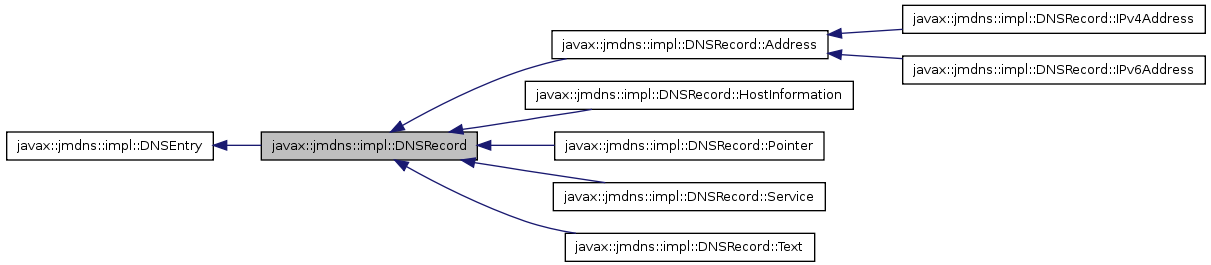
\includegraphics[width=17cm]{sprint5/jmdns.png}
	\caption{DNS record inherit graph.}
	\label{fig:DNS record inherit graph }
\end{figure}

It is important to say that this was not the case with all of the devices. Some of them, like Samsung Galaxy S2, was able to resolve detected services. It was clear that partially working solution is not good enough. After trying to fix the issue, and searching for answer on-line team decided to research additional alternative solutions.

\paragraph{Final fix}
Further research led to David Simmons multicast support application\footnote{\url{https://github.com/simmons/netlib}} on Android devices. His solution works on all Android devices beginning with system version 2.2. Big surprise was trying his application for detecting NSD created service, and JmDNS created services. It was working almost instantly with NSD, and all services ever created on test router were easy recognized and resolved. Since race condition were happening only on client devices, and empirically best match for registering/detecting and resolving service was NSD/netlib, team decided to keep different libraries that communication modules for server and client are based on. Final communication modules and their respective libraries are shown on Figure \ref{fig:Communication modules }

\begin{figure}[H]
	\centering
		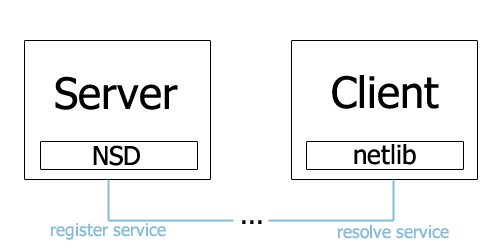
\includegraphics[width=9cm]{sprint5/com.png}
	\caption{Illustration of communication modules specific libraries.}
	\label{fig:Communication modules }
\end{figure}

\section{Customer feedback} \label{txt:sprint5_customerfeedback}
The main goal of this sprint was to collect as many devices as possible and use them to display various types of imagery including the equalizer effect which was chosen by the customer as the possibly most spectacular for the viewer. As the team encountered a few serious performance issues regarding the network communication and the time synchronization it was not able to deliver the demonstration video of the flawless animation. On the contrary due to technical issues the team was only able to display obviously not properly working animations on the borrowed phones. Nevertheless two demonstration videos were recorded and presented to the customer.

The customer were familiarized with the problems that lead to the faulty performance. He encouraged the team to prepare new demonstration videos that would show the imagery specifically adjusted in a way that it would not be obvious the team faces synchronization issues: lower fps, static images or abstract effects to list a few suggestions.

The first video presented to the customer can be found on YouTube under the name Demonstration - Equalizer [out of sync]\footnote{\url{http://www.youtube.com/watch?v=cDBcgPt1Sq8}}. 
The second video is published under the name Demonstation - Czech flag\footnote{\url{http://www.youtube.com/watch?v=MmTdFDsHTbk}}.

\section{Retrospective}
This section reflects on the past sprint. In order to learn from the mistakes done and thus to improve the workflow it is necessary to answer two essential questions: "What went well" and "What could be improved". Actual burn down chart is shown on Figure \ref{fig:Burn5 }

\begin{figure}[h]
	\centering
		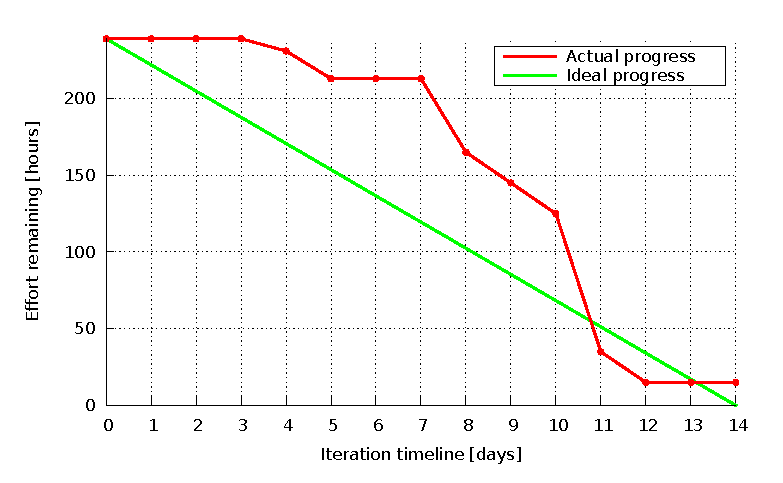
\includegraphics[width=14cm]{burndowns/sprint5.eps}
	\caption{Burn down chart.}
	\label{fig:Burn5 }
\end{figure}

\subsection{What went well}
Team collected more than enough devices for demonstration purposes. All devices have been collected from friends and colleagues since they were notified about recording date a whole week in advance, so there was no need to involve big companies in process. Recording equipment and room at the university were rented on time. 

All user stories considering implementation were finished on time, and occurred risk on communication module have been solved. Solving the issue was one of the main reasons for sufficient number of devices since new client module supports legacy devices. Detection algorithm speedup allowed better use of time devoted to recording. As a result of this improvements two demonstration videos have been recorded for the customer.


\subsection{What could be improved}
Connecting big number of devices(approximately 30) causes network low performance. For some messages it takes more than 3 sec to arrive to client. This make problems with device detection and synchronization. Team was aware of possible issue but didn't mark it as a high risk, because test was never launched on more than 3 devices as clients. As a result of this oversight equalizer video was hard to reproduce on clients and, after few attempts, not recorded at all. This could be avoided by thinking of networking issue as necessary to solve.

Team estimated that number of devices for recording the video will be bigger than 30. With this on mind most media that could be played was made for large-scale grid, including 25 pixels and more. After need to eliminate some of the devices not much of media left to be played. Team should prepare as diverse grids as possible in order to get better use of devices during next demonstration recording.

Also documentation user stories \textbf{D5.3} and \textbf{D5.4} were not completed because of underestimation of time needed. Team is reaching the last sprint, and it would be good if more time is spent on estimation because there is no more sprints to which user stories can be delegated.   


